%-----------------------------------------------------------------------------
%
%               Template for sigplanconf LaTeX Class
%
% Name:         sigplanconf-template.tex
%
% Purpose:      A template for sigplanconf.cls, which is a LaTeX 2e class
%               file for SIGPLAN conference proceedings.
%
% Guide:        Refer to "Author's Guide to the ACM SIGPLAN Class,"
%               sigplanconf-guide.pdf
%
% Author:       Paul C. Anagnostopoulos
%               Windfall Software
%               978 371-2316
%               paul@windfall.com
%
% Created:      15 February 2005
%
%-----------------------------------------------------------------------------


\documentclass{sigplanconf}

% The following \documentclass options may be useful:
%
% 10pt          To set in 10-point type instead of 9-point.
% 11pt          To set in 11-point type instead of 9-point.
% authoryear    To obtain author/year citation style instead of numeric.

\usepackage{amsmath}
\usepackage[pdftex]{graphicx}
\usepackage{listings}

\begin{document}

\conferenceinfo{WXYZ '05}{date, City.} 
\copyrightyear{2011} 
\copyrightdata{[to be supplied]} 

\titlebanner{banner above paper title}        % These are ignored unless
\preprintfooter{short description of paper}   % 'preprint' option specified.

\title{Python to Assembly Compilation}
\subtitle{With Reference Counting Garbage Collection}

\authorinfo{Brent Smith}
           {University of Colorado, Boulder}
           {brent.m.smith@colorado.edu}
\authorinfo{Robert Elsner}
           {University of Colorado, Boulder}
           {robert.elsner@colorado.edu}

\maketitle

\begin{abstract}
Garbage collection in high level languages has enabled increased programmer productivity, but at the cost of performance and ease of implementation for the language designer.  This paper will explore these trade-offs through an implementation of automatic garbage collection for a subset of the Python language.   Our implementation will extend an existing Python to x86 compiler to use reference counting garbage collection.  Reference counting is chosen for its ease of implementation, and because it is less invasive when one of the design goals is to integrate with assembly or C routines without extra intervention from the software developer.  We outline the changes to the existing compiler to enable reference counting, how the abstract syntax tree of the program is altered and what trade-offs are made with our design choices.
\end{abstract}

\category{D.1.5}{Programming Techniques}{Object-oriented Programming}
\category{D.3.3}{Programming Languages}{Language Constructs And Features-Dynamic Storage Management}
\category{D.3.4}{Programming Languages}{Processors- Memory Management (garbage collection)}
\category{D.4.2}{Operating Systems}{Storage Management-Garbage collection}

\terms
Management, Performance, Design, Languages, Algorithms

\keywords
memory management, garbage collection, reference counting, compilation, compilers, programming languages

\section{Introduction}

Python is a modern, high level language that uses dynamic typing and is run within an interpreter.  It manages memory for the programmer, and is considered by many to be a good "prototyping" language, in which programmers can quickly and easily develop an application.   Automatic memory management plays a large part in supporting this role, as it relieves the programmer from the tedious task of remembering when to de-allocate memory.  For language designers, deciding what form of memory management to incorporate into their language can be a difficult task.  The choice will depend on many factors, including the designer's vision on the general usefulness of the language, the environment where the language will be primary used, performance requirements, program semantics, integration with legacy systems and many other factors.  The choice also has significant implications on the implementation and therefore warrants careful consideration.  

There are currently two widely used strategies to perform automatic memory management.  One such strategy is tracing garbage collection, which periodically traverses the in-memory object graph starting from a currently reachable set of "root" objects.  This set of objects includes the set of all globals, as well as the objects which are referencable from the current stack frame.  Any objects that are traversed during this operation are considered reachable and therefore cannot be de-allocated.  Conversely, any objects not traversed are no longer reachable, and can be de-allocated.  The other primary strategy for automated memory management, is reference counting garbage collection. Reference counting works by keeping a count of references to a particular object.  References are tracked by incrementing and decrementing an object's reference count when an assignment to a pointer occurs, or when a pointer variable goes out of scope.  When the reference count reaches zero, it is safe to de-allocate the object.

The performance characteristics of each strategy can vary considerably, depending on implementation.   Tracing garbage collectors can sometimes be associated with long "pause" times, where application work must be paused to allow the entire contents of the heap to be scanned by the garbage collector.  These long pause times have largely been solved with new algorithms that improve upon the original naive mark-and-sweep algorithm.  It is typical that these algorithms tradeoff throughput for responsiveness.  However, these pause times can still be an issue, especially in real time systems, where a hard guarantees on latency are needed.  Reference counting has been discussed as a solution to this problem, but classic implementations of reference counting can have serious performance concerns when one de-allocation results in cascading de-allocations\cite{boehm}.  

Given a existing implementation of a Python to x86-assembly compiler which disregards all memory management, we explore the consequences of adding a reference counting garbage collector.  Our base Python-like language includes classes, objects, functions, lambdas, addition, unary subtraction, lists, dictionaries and integer primitives.  The remainder of the paper is organized as follows.  Section~\ref{sec:related} discusses related work.  Section~\ref{sec:implementation} discusses the implementation of reference counting for our compiler.  Section~\ref{sec:results} evaluates our compiler for performance and correctness.  Section~\ref{sec:future} discusses potential future work.  Finally, section~\ref{sec:conclusion} concludes.


\section{Related Work}
\label{sec:related}
In general a reference count garbage collector will have shorter pause times for the garbage collection phase, but will incur a higher performance penalty \cite{joisha}\cite{blackburn}.  Reference-counting collectors have been implemented which defer the de-allocation, called lazy reference-counting, to some later time and some improvements on such strategies have been made \cite{boehm}.  Without extra work a strictly reference-counting collector will leak memory when references contain cycles, and multiple algorithms have been presented as solutions to this problem. \textit{Citation?}

One potential advantage that reference-counting garbage collectors have is the ability to be implemented in hardware \cite{joao}.  Given the significant cost of garbage collection \cite{hertz} any hardware assisted acceleration would be highly desirable if it is flexible enough to adapt across multiple garbage collection techniques. 

Real-time systems are rarely implemented in languages which are garbage collected, but reference-counting garbage collection has been adapted to hard real-time systems \cite{ritzaou}.  Due to immediate knowledge that an object is no longer in use reference counting garbage collection can allow for destructors or finalizers to be run immediately which can enhance the clean up of system resources.

\par
\section{Implementation}
\label{sec:implementation}

We develop a base compiler which generates x86 assembly code and then alter the compiler to include reference counting and garbage collection.

\subsection{Language}
A subset of Python has been chosen which includes functions, objects, lambdas, and the primitives integer, boolean.  We implement this as a reference compiler which is extended to include reference counting.  This language has no built in parallelism but Levanoni, et. al. have shown that reference counting is a valid approach for multprocessor systems.\cite{levanoni}
\par
Starting from our reference compiler, we treat any object which is not an integer or boolean primitive as a C structure.  This structure was modified to include a reference counter and in all places where such a structure was allocated we converted the allocation to use a statistics tracking allocator and set the reference count to an initial value of 0.
\par
We chose to implement our own memory routines primarily to investigate object lifetime (initial allocation time and final de-allocation time) as well as allow us the ability to detect memory leaks.  Since every allocation of an object in our language uses this wrapper we know exactly how much memory has been allocated and what objects were never de-allocated.
\par
The basic premise of such routines is to wrap the provided malloc and free, request slightly more memory than required.  That extra memory is what where the reference counter is stored and the pointer location is returned which skips the counter.  The memory routines also create a linked list to track all of the allocations in a structure for statistics gathering and leak detection.
\begin{figure}
\begin{center}
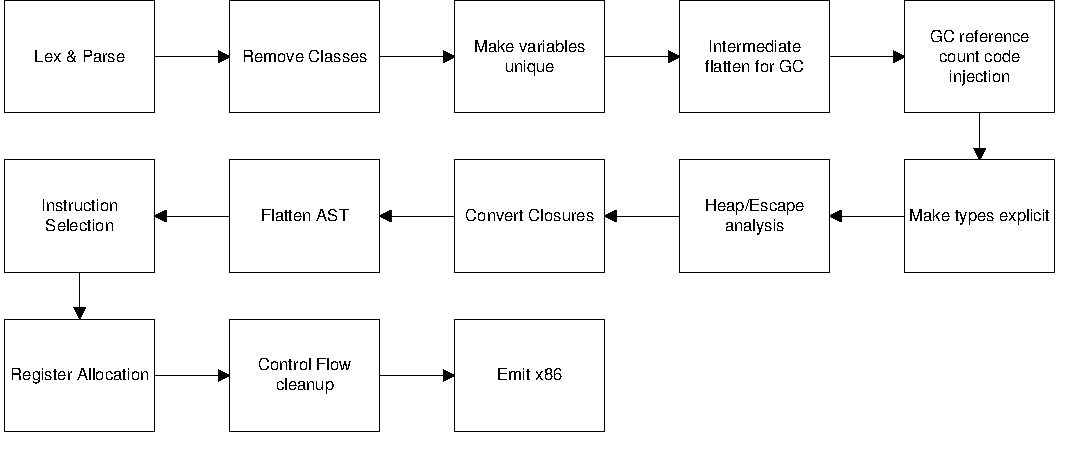
\includegraphics[scale=0.48]{compiler_flow.pdf}
\end{center}
\caption{Compiler Architecture}
\label{fig-comparch}
\end{figure}

\subsection{Compiler Flow}
Refer to Figure~\ref{fig-comparch} for the compiler data flow.  Each stage operates on an abstract syntax tree, the relevant new stages are the garbage collection flattening stage and the reference count AST transformation stage.

\subsection{Syntax Tree Modifications}

\subsubsection{New compiler stages}
We added two new stages to our reference compiler.  The first stage is a modified flattening stage, which produces a flattened AST to aid in the reference determination.  The next stage is the actual reference determination and AST transformation, where the compiler determines what variables will be objects and when assignments happen and adds appropriate calls to increment and decrement the reference counter of the object as needed.
\par
Our initial assumption was that we could easily add the increment and decrement reference counter operations in the reference compilers flatten stage, however because this stage is after type explication and there are variables created which do not correspond to a type in the language the pre-flatten stage was necessary.  This stage converts all expressions in to assignments to temporary variables.  At this stage we know every expression is operating on types.

\subsubsection{Analysis on when to decrement an object reference}
The next new stage is the reference counting AST transformation.  In this stage we take the flattened tree and look for assignments which are setting list elements, dictionary values, class attributes, object attributes or variables.  The compiler determines what variables are created in the current scope and injects code at the beginning of that scope to set the value initially.  We decided on this approach to simplify determining when an object is first assigned and this allows us to simply decrement the reference counter to the object before an assign, regardless of the variables state.

\subsubsection{Temporary Variables}
The compiler creates temporary variables in a number of situations (namely function calls and as a result of flattened expressions).  These temporary variables need not hang on to their memory reference past the next assignment to the actual result variable.  Any temporary variable is dereferenced immediately at the end of the current scope if it is not the variable being returned.  If it is the return variable we ignore decrementing the reference on this variable, thereby assuring the caller that the object returned is correctly reference counted for its assignment.  If we had decremented the reference counter, due to the immediate nature of garbage collection, we would have been returning a value which did not point to an allocated memory region.

\subsection{Runtime Modifications}
Our runtime consisted of C functions which took care of allocating and initializing memory for a new object of a given type.  The obvious modifications included setting the reference counter initially to zero and creating a number of free functions to free each type of object.
\par
In the free\emph{\_type} functions it was necessary to add further calls to decrement the reference counter of any objects referenced by the type.  For a list list we iterate the values contained in the list, decrementing their reference (which can result in freeing that object).  For a dictionary we decrement the reference counter on keys as well as values contained in the dictionary, since both can be objects.

\subsection{Interesting Problems}
We encountered a number of interesting questions during this implementation and summarize them below.

\subsubsection{Addition of Lists}
In the current runtime an entirely new list is created when two lists are added together.  At the assignment level our compiler can determine (due to the flattened structure) that the left-hand-side and the right-hand-side of the addition need their reference counters manipulated, however the assignment from an addition to a list creates an entirely new list which should properly increment the reference counter to all objects in both lists.

\subsubsection{Variable Assignment}
We wanted a simple way to determine when to decrement an objects reference counter.  Our first implementation was to add a call to decrement the counter before every assignment.  However, because a variable can be created at any point in program execution we couldn't just blindly decrement the counter of an object since the variable will be uninitialized, and could be pointing at memory that makes it look like an object or accidentally references an object.
\par
The solution we took makes a slight modification to program behaviour, but we feel it is an acceptable trade-off.  In every scope, the compiler adds an immediate assignment as the first instructions.  This assignment is to a primitive, so the cost is minimal and then a decrement on the reference counter amounts to a function call with a no-op.  This function call overhead could potentially be avoided by adding code to check if the variable points to an object or a primitive and is a future enhancement for performance.  A program which used uninitialized (or declared) variables for program flow control would then have its runtime semantics changed.  We felt this was a sufficient trade off since such use of an exception for program flow control is frowned upon in practice and the benefit to our design was an obvious positive.


\subsection{Assembly Output}
We modified the x86 assembly to include calls to set up our memory tracking system and print statistics at the end of the program.  Running analysis tools such as valgrind on our programs before and after shows the obvious gain of going from every memory allocation leaks to zero leaks.

\section{Results}
\label{sec:results}

\subsection{Execution}

\subsection{Memory}

\subsubsection{Valgrind results}
For the trivial program
\begin{verbatim}
i = 0
list = []

while i !=  10000:
    list = list + [[i]]
    i = i + 1

\end{verbatim}
Without any garbage collection, valgrind reports 
\begin{verbatim}
==23467== LEAK SUMMARY:
==23467==    definitely lost: 560,028 bytes in 20,001 blocks
==23467==    indirectly lost: 199,004,992 bytes in 20,191 blocks
==23467==      possibly lost: 1,375,008 bytes in 19,810 blocks
\end{verbatim}
With our reference counting for the same program
\begin{verbatim}
==23831== LEAK SUMMARY:
==23831==    definitely lost: 0 bytes in 0 blocks
==23831==    indirectly lost: 0 bytes in 0 blocks
==23831==      possibly lost: 0 bytes in 0 blocks
\end{verbatim}

\section{Future work}
\label{sec:future}

\section{Conclusions}
\label{sec:conclusion}

\subsection{Disadvantages}

\subsection{Advantages}

\appendix
\section{Appendix Title}

This is the text of the appendix, if you need one.

\acks

We would like to thank Jeremy Siek and Evan Chang for the course notes from which the compiler design is derived.

% We recommend abbrvnat bibliography style.

\bibliographystyle{abbrvnat}

% The bibliography should be embedded for final submission.

\begin{thebibliography}{}
\softraggedright
\bibitem{joisha}
Pramod G. Joisha. 2006. Compiler optimizations for nondeferred reference: counting garbage collection. In Proceedings of the 5th international symposium on Memory management (ISMM '06). ACM, New York, NY, USA, 150-161. DOI=10.1145/1133956.1133976

\bibitem{blackburn}
Stephen M. Blackburn and Kathryn S. McKinley. 2003. Ulterior reference counting: fast garbage collection without a long wait. In Proceedings of the 18th annual ACM SIGPLAN conference on Object-oriented programing, systems, languages, and applications (OOPSLA '03). ACM, New York, NY, USA, 344-358. DOI=10.1145/949305.949336

\bibitem{boehm}
Hans-J. Boehm. 2004. The space cost of lazy reference counting. In Proceedings of the 31st ACM SIGPLAN-SIGACT symposium on Principles of programming languages (POPL '04). ACM, New York, NY, USA, 210-219. DOI=10.1145/964001.964019 

\bibitem{joao}
José A. Joao, Onur Mutlu, and Yale N. Patt. 2009. Flexible reference-counting-based hardware acceleration for garbage collection. In Proceedings of the 36th annual international symposium on Computer architecture (ISCA '09). ACM, New York, NY, USA, 418-428. DOI=10.1145/1555754.1555806

\bibitem{hertz}
Matthew Hertz and Emery D. Berger. 2005. Quantifying the performance of garbage collection vs. explicit memory management. In Proceedings of the 20th annual ACM SIGPLAN conference on Object-oriented programming, systems, languages, and applications (OOPSLA '05). ACM, New York, NY, USA, 313-326. DOI=10.1145/1094811.1094836  

\bibitem{levanoni}
Yossi Levanoni and Erez Petrank. 2006. An on-the-fly reference-counting garbage collector for java. ACM Trans. Program. Lang. Syst. 28, 1 (January 2006), 1-69. DOI=10.1145/1111596.1111597 

\bibitem{ritzau}
Tobias Ritzau. 1999.  Real-Time Reference Counting in RT-Java

\end{thebibliography}

\end{document}
